All arms end after the same 20 post-warmup epochs; $a=100$ and $a=20$ specify nominal ramp horizons within that window. All six background--seed pairs pass initial-state, warmup-boundary,
minibatch, refit-subset and update-count gates. Both cap-5 arms bind on every
recorded coupling-window batch and have zero batches with an effective
mixture gradient. Their final latent arrays are byte-identical to the
uncoupled anchor in all six pairs. This establishes a cap-mediated freeze
for cap 5 in this experiment. It does not establish a freeze for an
arbitrarily large finite cap.

Removing the cap lowers edge survival at each fixed nominal ramp horizon in
all six pairs (Figure~\ref{fig:factorial}). Reducing the nominal horizon from $a=100$ to
$a=20$ within the same 20-epoch window leaves the capped latents unchanged but further lowers edge survival in
all six uncapped pairs. The historical uncapped difference therefore included
an exposure effect as well as cap removal. Table~\ref{tab:factorial} reports
all arms by background. Between 140 and 192 batches per uncapped $w=1$ arm
have both a nonzero mixture gradient and a nonzero weight, compared with
zero for capped arms and the anchor. Nominal ramp horizon alone does not
count effective interventions; the lower clip can also suppress the gradient.

The Setty branch probe separates the uncapped schedules. Its three values
are $0.653/0.718/0.684$ for the anchor and both capped arms,
$0.793/0.511/0.604$ for uncapped $a=100$, and
$-0.555/-0.266/0.347$ for uncapped $a=20$.
The slower uncapped schedule includes one improvement relative to the anchor;
a claim that removing the cap always lowers this branch score is unsupported.
All three faster-schedule values are lower than their paired slower-schedule
values. There is no Palantir endpoint for Endo.

The installed and terminal mixtures often disagree markedly in effective
occupancy (Table~\ref{tab:factorial}). For example, Setty uncapped $a=20$ has training occupancy $15.28/8.86/6.35$ but terminal observer occupancy
$11.72/49.80/49.81$. Both parameter sets and their conditional probabilities
are saved. They differ in refit time, sample size and installed precision
handling, so these are different estimators, not alternative counts of a
known biological state population.

An independent archive audit finds nonconvergence flags in 46 of the 60 recorded training refits (two per endpoint arm). Counts include repeated matched fits. This limits mixture-fit and occupancy interpretation, while the saved bound activity and exact capped-anchor equality remain directly checkable.

An initial production attempt stopped at the warmup-boundary equality gate
before any endpoint: loading an AdamW state without copying its tensors
mutated the reusable source state. The corrected driver deep-copies the
optimizer state before every fork. The failed attempt's 2,890 optimizer
updates are retained separately, as are 29 smoke updates and 60 successful
gate-probe updates. The completed experiment executes 24,360 unique scientific
updates by sharing warmup; the thirty endpoint histories together represent
87,000 updates. The failed attempt contributes no scientific endpoint.

\begin{figure}[htbp]\centering
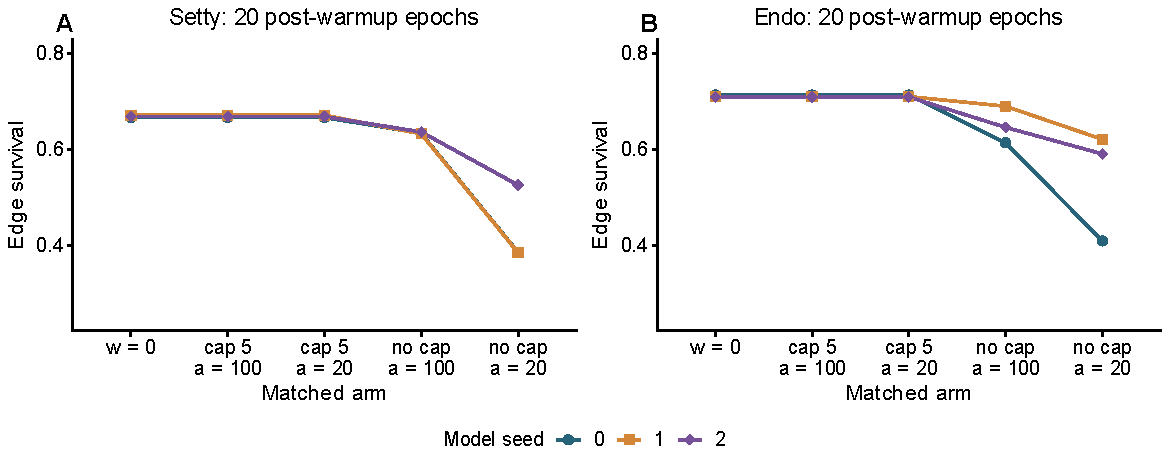
\includegraphics[width=\textwidth,height=0.70\textheight,keepaspectratio]{figures/factorial_edge.pdf}
\caption{All thirty matched factorial endpoints at epoch 200.
A: Setty; B: Endo. Edge survival compares each latent with PCA-50 neighbours of the same 450 or 380 held-out cells. Five categories cross cap 5/no cap with nominal horizon $a=100/20$ and include a $w=0$ anchor. Color/shape identify seeds in the shared key. Lines join matched categorical arms, not a continuous dose. Capped arms coincide with the anchor but retain separate records. Each arm receives twenty post-warmup epochs. There are six shared histories, with no seed averaging or error bars.}
\label{fig:factorial}\end{figure}

\begin{table}[htbp]\centering\small
\caption{Matched factorial summaries across three model seeds. Edge reports mean $\pm$ sample SD. $K_T$ and $K_O$ report seed means of last training-refit and terminal-observer effective occupancy, respectively. Gradient counts give the observed seed range of batches
with a nonzero mixture gradient and positive effective weight. They are not
independent biological observations.}
\label{tab:factorial}
\begin{tabular}{llrrrr}\toprule
Background & Arm & Edge, mean $\pm$ SD & $K_T$ & $K_O$ & Active batches\\\midrule
Setty & $w=0$ & $0.668\pm0.002$ & 9.27 & 9.48 & 0--0 \\
Setty & $c=5,a=100$ & $0.668\pm0.002$ & 9.27 & 9.48 & 0--0 \\
Setty & $c=5,a=20$ & $0.668\pm0.002$ & 9.27 & 9.48 & 0--0 \\
Setty & $c=\infty,a=100$ & $0.634\pm0.002$ & 24.04 & 48.83 & 179--184 \\
Setty & $c=\infty,a=20$ & $0.432\pm0.081$ & 10.16 & 37.11 & 175--192 \\
Endo & $w=0$ & $0.711\pm0.002$ & 8.86 & 8.68 & 0--0 \\
Endo & $c=5,a=100$ & $0.711\pm0.002$ & 8.86 & 8.68 & 0--0 \\
Endo & $c=5,a=20$ & $0.711\pm0.002$ & 8.86 & 8.68 & 0--0 \\
Endo & $c=\infty,a=100$ & $0.650\pm0.038$ & 31.02 & 48.16 & 148--155 \\
Endo & $c=\infty,a=20$ & $0.540\pm0.114$ & 23.86 & 35.49 & 140--157 \\
\bottomrule\end{tabular}\end{table}
